\subsection{Implementation}
\label{sec:wave-implementation}

To implement a wave system, we created a class called Wave which handles the 
spawning of new units and incrementing the wave counter and stat modifier.
This class and its relations are shown in \cref{fig:wave}.

\begin{figure}[!htb]
    \centering
    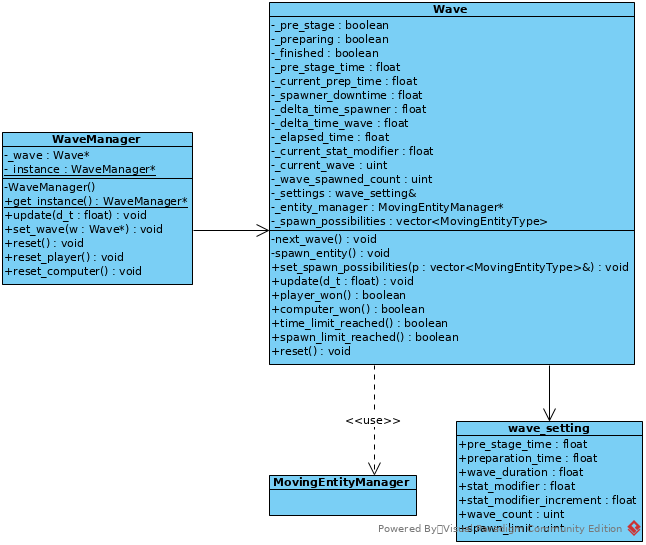
\includegraphics[scale=0.75]{res/wave.png}
    \caption{Wave class and relations.}\label{fig:wave}
\end{figure}

Every update cycle, the update method of wave gets called. In this update 
method we check whether the wave is in a preparation state. If it is we 
simply decrement the preparation time variable with the delta time passed to 
the update method. If we're in a spawning state, we check whether we've 
already spawned the maximum amount of entities for this wave. If not, we spawn 
an entity, increment the entity counter and decrement the spawning timer.

Once we've checked if we need to spawn an entity, we need to check if we 
reached the next wave. If so, we increment the wave counter and the stat 
modifier and we reset the amount of entities spawned in the wave so that we 
can spawn new entities this wave.

The code for this is shown in \cref{lst:wave-update}.
\\
\begin{lstlisting}[caption={Spawning entities and next wave.},
label={lst:wave-update}]
if(!_preparing) {
    _delta_time_wave += delta;
    _delta_time_spawner += delta;
    _elapsed_time += delta;
    if(!spawn_limit_reached()) {
        spawn_entity();
    } else if(spawn_limit_reached() && _current_wave < _settings.wave_count) {
        next_wave();
    }
}
\end{lstlisting}
